%%\documentclass{nature}
\documentclass{article}
\usepackage{xr}
\bibliographystyle{natbib}
\renewcommand{\baselinestretch}{1.4} 
\usepackage{graphicx}
\usepackage{bm}
\usepackage{lineno}
\usepackage{natbib}
\usepackage{setspace}
\usepackage{authblk}
\usepackage{xcolor}

\linenumbers


%% external tex files
%%\externaldocument{figure1_runtimes}
%%\externaldocument{figure2_powerFDRmultiple}
%%\externaldocument{figure3_mouse}

\externaldocument{supmaterials}

\begin{document}

\title{Eagle: multi-locus association mapping on a genome-wide scale made routine}
\author[1]{Andrew W. George}
\author[2]{Arunas Verbyla}
\author[3]{Joshua Bowden}
\affil[1]{Data61, CSIRO, Brisbane, 4102, Australia.}
\affil[2]{Data61, CSIRO, Atherton, 4883, Australia.}
\affil[3]{IM \&T, CSIRO, Brisbane, 4067, Australia}
\date{}


\maketitle


%% New commands ... 
\newcommand{\bwidetildea}{\widetilde{\bm{a}}}
\newcommand{\bu}{\bm{u}}
\newcommand{\be}{\bm{e}}
\newcommand{\btau}{\bm{\tau}}
\newcommand{\ba}{\bm{a}}
\newcommand{\bzero}{\bm{0}}
\newcommand{\bI}{\bm{I}}
\newcommand{\bX}{\bm{X}}
\newcommand{\by}{\bm{y}}
\newcommand{\bZ}{\bm{Z}}
\newcommand{\bM}{\bm{M}}
\newcommand{\bmm}{\bm{m}}



\begin{abstract} \noindent
\setstretch{1.6}{
{\bf Motivation:} We present Eagle, a new method for multi-locus association mapping. The motivation for developing Eagle was to make multi-locus association mapping "easy" and the method-of-choice. Eagle's strengths are that it a. is considerably more powerful than single-locus association mapping b. does not suffer from multiple testing issues c. gives results that are immediately interpretable and d. has a computational footprint comparable to single-locus association mapping. \\
{\bf Results:} By conducting a large simulation study, we will show that Eagle finds true and avoids false SNP-trait associations better than competing single- and multi-locus methods. We also analyse data from a published mouse study. Eagle found over 100\% more validated findings than the state-of-the-art single-locus method.  \\
{\bf Availability and Implementation:} Eagle has been implemented as an R package, with a web-based Graphical User Interface (GUI) for users less familiar with R. It is freely available via the CRAN website  at https://cran.r-project.org.  \\
{\bf Contact:} andrew.george@csiro.au
}
\end{abstract}



\section{Introduction}
Over the past decade,  genome-wide association studies (GWASs) have changed considerably in both their analysis and design. Early studies
 followed a case-control design. Association mapping methods were no more complicated than contingency table tests or simple 
linear regression. These designs though had a tendency to yield spurious findings if there was unrecognised population stratification 
\citep{cardon2003population}. This prompted a shift towards family-based designs and score tests, such as the transmission/disequilibrium test (TDT)  and its variants \citep{spielman1996tdt}. Today, instead of by design, it is through statistical modelling that we account for the effects of population stratification \citep{price2010new}. This has meant that data can be collected from general populations, even if these populations are highly structured. Analysis via sophisticated association mapping methods, such as linear mixed model based approaches,  is now almost routine  \citep{yu2006unified,zhao2007arabidopsis}.




What has not changed is that it remains common practice to analyse genome-wide association study (GWAS) data on a locus-by-locus basis. This is despite there being several significant problems with analysing data in this way. 
First, \textcolor{red}{ for each SNP, a hypothesis test is performed. The null hypothesis is that  there is no association between the SNP and trait. 
The alternative is that the SNP is in association with the trait. It is straight forward to guard against wrongly rejecting the null 
hypothesis (or making a type 1 error) if only a single hypothesis test is being performed. However, the analysis of GWAS data 
with locus-by-locus methods necessitates  conducting a large number of correlated hypothesis tests, simultaneously. 
 This leads to an increased risk of type 1 errors.  To deal with this challenge, many different solutions have been offered 
 \citep{storey2003statistical, li2005adjusting, de2005efficiency}.  Second, 
the aim of association mapping is to identify regions of the genome that house genes that are influencing a trait. 
The identification of these regions from these analyses is not always straightforward. GWAS results are reported, typically, via Manhattan plots 
that plot the -log$_{10}$ of the $p$ value for each locus against the map position of the locus. The $p$ value is obtained from the hypothesis test. 
The location of peaks in this plot identify genomic 
regions of interest. Inferring the exact number of regions though can be difficult if the peaks are not well separated. }
 Third, many of the traits whose genetic secrets we are trying to discover are complex. There will be multiple SNPs in linkage disequilibrium with genes that are influencing the trait. Yet, a locus-by-locus mapping approach only assesses the evidence for association between a single marker locus and trait.

It is somewhat surprising then that multi-locus association mapping methods haven't attracted more attention. Methods based on 
regularisation techniques, such as ridge regression \citep{shen2013novel}  and lasso \citep{rakitsch2013lasso}, measure all locus-trait associations simultaneously. These techniques though are computationally demanding. \textcolor{red}{Also, the strength of association is not measured by a $p$ value but by the size of the regression coefficient for the SNP in the model. Further processing is required before the results can be interpreted \citep{cho2010joint, rakitsch2013lasso}}.
More recently, associations have started to be mapped with random forests \citep{szymczak2016r2vim}. Similar to regularisation techniques though, it is not clear how to infer genomic regions of interest from their findings. A multi-locus method that does show promise is the multiple-locus linear mixed model method \citep{segura2012efficient}. The best multi-locus model is built with forward and backward stepwise selection. 
Results are immediately interpretable \textcolor{red}{in that the SNP closest to the genes underlying the trait are identified} 
but computation does become challenging for large datasets. 

In this paper, we present our new multi-locus method for genome-wide association mapping, which we are calling Eagle. 
Eagle combines the strength of regularisation techniques (being able to fit all SNP-trait associations jointly), with forward selection giving easy-to-interpret threshold-free results.   We are able to achieve a computational performance similar to the fastest single-locus linear mixed model implementations 
through a dimension reduction step.
Our aim was to make multi-locus association mapping on a genome-wide scale routine. To this end, we have implemented Eagle 
within an R package of the same name. 
Our package accepts marker data of different 
formats,  can handle data larger than a computer's  memory capacity, and makes heavy use of 
parallel computing for computation when available.  










\section{Methods}

\subsection{Mouse Data}

The data were obtained from a large genome-wide association study that was performed in outbred mice \citep{nicod2016genome}. 
Phenotypic and genotypic data were available on 1,887 adult mice. 
The phenotypic data included raw and adjusted (for fixed effects) measurements from 200 behavioural, tissue, and physiological traits.  
Of these traits, 
43 yielded SNP-trait associations that could be corroborated through other independent published work. It was these 
43 traits that were the focus of our real data analyses. As in the original study  \citep{nicod2016genome}, our analyses 
were based on the adjusted traits.
Genotypic data were available on \textcolor{red}{359,559} (353,697 autosomal) SNPs in the 
form of marker dosages (expected allele counts that ranged from zero to one). All missing data had been imputed. 
We converted the dosages into discrete genotypes 
by clustering around 0, 0.5, and 1, corresponding to SNP genotypes AA, AB, and BB, respectively. 
We focused our analyses on the autosomal SNPs.




\subsection{Eagle Approach for Multi-locus Association Mapping}
\label{subsection:Eagle}

\textcolor{red}{
Eagle is a method for multi-locus association mapping on a genome-wide scale. It is based on linear mixed models. It differs from most other single- and multi-locus association mapping methods in that Eagle treats association mapping as a model selection problem \citep{ball2001bayesian,broman2002model,yi2005bayesian}. 
The "best" model is found via forward selection. It makes use of a modified form of the Bayesian information criterion, BIC, for model selection.
A "best" model is built iteratively. At each iteration, a hypothesis test is performed. 
Only a small number of iterations are needed in building the "best" model.  Consequently, 
Eagle does not suffer from multiple testing issues.
In contrast,  for single-locus methods, multiple testing is an 
issue because each SNP is assessed separately, culminating in the need for a large number of hypothesis tests to be  performed. 
Eagle 
reports as its findings only those SNPs that are in strongest linkage disequilibrium with  the genes influencing a trait. }
The methodological foundation for Eagle comes from a whole-genome linkage analysis method that was developed for mapping 
quantitative trait loci in experimental crosses \citep{verbyla2007analysis}.


Let $S = \{ S_1, S_2, \ldots, S_s\}$ be a set of $s$ ordinal numbers where $S_k$ is the $S_k$th ordered SNP that was 
selected in the $k$th iteration of the model building process. Suppose three iterations  $(s=3)$
have been performed and say the 500023rd, 15th, and 420th
SNP were selected. Then $S=\{500023, 15, 420\}$. 
Let $\by^{(n \; \times \;1)}$ be a vector containing $n$ measurements of the quantitative trait. 
Let $\bM^{(n_g \; \times \; L)} = [\bmm_1 \bmm_2 \ldots \bmm_L]$ be a matrix containing the genotype data which have been collected 
from $L$ loci that span the genome on $n_g$ groups/lines/strains.  Here, $n \geq n_g$ meaning that a single or several trait measurements 
may be taken of the same group/line/strain. 
 It is common for the columns of $\bM$ to be in map order but this is not a requirement. 
The vector $\bmm_j^{(n_g \; \times \; 1)}$ contains the genotypes for the $j$th SNP. 
The genotypes are coded as -1, 0, and 1 corresponding to SNP genotypes AA, AB, and BB, respectively. 

The specifics of the Eagle method are as follows. 
Eagle builds the "best" model iteratively, via forward selection. 
Suppose $s$ iterations of our model building process have already been performed. This means $s$ SNP-trait 
associations have been identified.  It also means that $s$ separate genomic regions of interest have been found.  
To perform the $s+1$th  iteration, we first fit the current model to the data. 
The (current) model is of the form 
\begin{equation}
\label{eq1}
\by = \bX \btau + \bZ \bu_g + \be
\end{equation}
where 
$\bX^{(n \; \times \; p)}$ and $\bZ^{( n \; \times \; n_g)}$ are known design matrices with $\bX$ being of full rank and $\bZ$ 
containing zeros and ones that assign the appropriate genetic effect to each measurement. 
The vector 
$\btau^{(p \; \times \; 1)}$ has $p$ fixed effects parameters including the intercept. The vector 
$\bu_g^{(n_g \; \times \; 1)}$ contains the 
genetic effects. The vector of residuals is 
$\be^{(n \; \times \;1)}$ whose distribution is assumed to follow $N(\bzero, \sigma^2_e \bI^{(n \; \times \; n)})$. 
So far,  this model differs little from standard linear mixed models for association mapping \citep{yu2006unified,zhao2007arabidopsis} 
However, 
it is how we specify $\bu_g$ that distinguishes our model from the others. 

The genetic effects $\bu_g$ are modelled as 
\begin{equation}
\label{eq2}
\bu_g = \sum_{k=1}^s  \bmm_{S_k} a_{S_k} +\bM_{-S} \ba_{-S}
\end{equation}
where $\bmm_{S_k}^{(n_g \; \times \; 1)}$ is the vector of genotypes for the  $k$th selected SNP, 
$a_{S_k}$ is the additive effect of the $k$th selected SNP, $\bM_{-S}^{(b \; \times \; L-s)}$ is the matrix of  SNP genotypes 
with the data for the SNP in $S$ removed,  and $\ba_{-S}^{(L-s \; \times  \; 1)}$ is a random effect whose distribution is 
$\ba_{-S} \sim N(\bzero, \sigma_a^2 \bI^{(L-s \; \times \;  L-s)})$. 
The terms in the summation on the left hand side are fixed effects.   They account 
for the additive effects of those SNPs that have been found to be in association with the trait. The other term is a random effect. 
It accounts for the joint effect of the yet-to-be-identified SNP that are in association with the trait. 
This is a simple genetic model but it 
is effective for discovering SNP-trait associations. 


Second, we estimate the parameters of (\ref{eq1}) and (\ref{eq2}) via \textcolor{red}{restricted} maximum likelihood (REML).  For complex models, REML
can be computationally demanding. However, our model only contains a single random effect ($\ba_{-S}$). Here, highly efficient single-dimension 
optimisation via spectral decomposition is possible \citep{kang2008efficient}. 

Third, we identify the $(s+1)$th SNP that is in strongest association with the trait, based on the maximum score statistic
$t_j^2 = \frac{ \widetilde{a} _j^2}{\textrm{var}(\widetilde{a}_j)}$ where $\widetilde{a}_j$ is the best linear unbiased predictor (BLUP), 
and $\textrm{var}(\widetilde{a}_j)$ is its variance. This statistic is not only appealing intuitively, where we 
identify a SNP based on its (random) effect size and accuracy, but is justifiable, theoretically \citep{verbyla2012rwgaim}.

Fourth, we determine the importance of the $(s+1)$th selected SNP via a model selection strategy  \citep{verbyla2007analysis}. 
We begin by reforming (\ref{eq2}) where $S$ now contains the $s + 1$ selected SNP.  We then fit this new model to the data
via maximum likelihood and calculate its extended Bayesian information criteria (extBIC) \citep{chen2008extended}.  The 
extBIC is a model selection measure that takes into account the number of unknown parameters and the complexity 
of the model space.  It is well suited to the model selection problem in genome-wide association studies \citep{chen2008extended}. 
It is different to the model selection measure used in  \citep{verbyla2007analysis}.
If this new model has a larger extBIC than the current model, then the $s+1$th selected SNP is added to 
the current model and the above process is repeated. If this new model has a smaller extBIC than the current model, then the 
model building process is complete. The set of SNP in strongest association with the trait is the $s$ SNPs previously identified. 

\subsubsection {Reducing the dimension of the model:} 

In practice, estimating the parameters of (\ref{eq2}) can be demanding, computationally. 
The vector $\ba_{-S}$ has $L-s$ random effects where in modern genome-wide association studies, 
$L$, the number of SNPs, can be extremely large.  An alternative model is given by 
Verbyla \citep{verbyla2012rwgaim,verbyla2014whole}. 
They show how to reformulate (\ref{eq2}) to be a model with a random effect with only $n$ elements
\begin{equation}
\label{eq3}
\bu_g = \sum_{k=1}^s  \bmm_{S_k} a_{S_k} + (\bM_{-S} \bM_{-S}^T)^{1/2} \ba^*_{-S}
\end{equation}
where $\ba^* \sim N(\bzero, \sigma_a^2 \bI^{(n_g \; \times \;  n_g)})$, and 
$(\bM_{-S} \bM_{-S}^T)^{1/2}$ can be calculated via singular value decomposition \citep{golub2012matrix}.  
Although it may not be obvious, the two models are equivalent, 
having identical variance structures. Yet, the computational cost of model (\ref{eq3}) compared to 
model (\ref{eq2}) is much less, due to the random term in model (\ref{eq3}) having only $n$ instead of $L-s$ 
effects needing estimating. 

Verbyla \citep{verbyla2012rwgaim,verbyla2014whole} go on to show how to recover $\bwidetildea$ from estimates from model  (\ref{eq3})  with 
\begin{equation}
\bwidetildea = \left [ \bM_{-S}^T (\bM_{-S} \bM_{-S}^T)^{-1/2} \right ] \bwidetildea^*
\end{equation}
where its variance matrix is
\begin{equation}
\label{eq4}
\textrm{var}(\bwidetildea) = \bM_{-S}^T (\bM_{-S} \bM_{-S}^T)^{-1/2} \textrm{var}(\bwidetildea^*) (\bM_{-S} \bM_{-S}^T)^{-1/2} \bM_{-S}
\end{equation}
These values are needed in order to calculate the score statistic $t_j^2$ for identifying the SNP in strongest association with the trait. 
Fortunately, when calculating $t_j^2$, only the diagonal elements of the variance matrix are needed which simplifies the  calculation 
of (\ref{eq4}). 

%%\iffalse 

\subsection{Comparison Methods}

 \subsubsection{ Multi-locus methods:} We compare the computational and statistical performance of Eagle against five multi-locus methods. \textcolor{red}{They are bigRR  \citep{shen2013novel}, LMM-Lasso \citep{rakitsch2013lasso}, glmnet \citep{Friedman2010glmnet}, 
MLMM \citep{segura2012efficient}, and r2VIM \citep{szymczak2016r2vim}}.  All but glmnet have been purposely designed for genome-wide association mapping. 
BigRR, LMM-Lasso, and glmnet are regression-based regularisation 
methods. BigRR is based on generalised ridge regression, LMM-Lasso is based on lasso, and glmnet is based on elastic net. 
Regularisation methods make parameter estimation possible in models  where the number of predictors is far greater than the number of samples. 
They allow the strength of association between all the SNPs and trait to be measured within a single model, simultaneously. 
A limitation of these methods though is that the statistical significance of the SNP effects cannot be easily determined. 
 Due to the adaptive nature of the estimation procedures, to do this 
analytically is challenging and is an area of active research \citep{lockhart2014significance}. Instead, we calculate significance empirically via 
stability selection (see below). 

MLMM is closest in philosophy to Eagle. It too is based on building the best model via \textcolor{red}{stepwise} selection, 
within  a linear mixed model framework, and uses the 
extBIC as one of its model selection criterion. However, there are differences between the two methods. 
MLMM does not make use of dimension reduction. \textcolor{red}{Also, how SNP are selected to enter the model differs between the 
two methods. 
Eagle identifies a SNP of interest from its score statistic (see Section \ref{subsection:Eagle} for details).  This score statistic was originally developed for 
outlier detection in linear (mixed) models but it is being used by Eagle to identify 
SNP with unusually large random effects. MLMM instead uses 
the statistical significance of a SNP,  when treated as a fixed effect in the model. This involves fitting a separate linear mixed model for each candidate SNP, a potentially
computationally expensive exercise. However, MLMM does this in a clever and efficient way via the Gram-Schmidt process. 
Both are R packages but there is a significant difference in computational performance (see Results). 
Note, even though a hypothesis test is being performed for each SNP by MLMM, it does not suffer from multiple testing issues. 
Neither the null nor the alternative hypothesis is being accepted or rejected. Only the hypothesis yielding the most significant association is 
of interest. }



  
R2VIM differs to the other four methods in that it is a non-parametric model-free approach. It implements  
random forests but where multiple parallel runs are performed. Each run leads to 
different random forests being created.  A relative importance score is calculated, within a run,  for each SNP. This is done by dividing a SNP's 
importance score by the minimum importance score observed across all the SNPs within a run. 
Only those SNPs with relative importance scores above a certain threshold across all the runs are deemed to be significant. 
Unfortunately, the relationship between threshold value and false positive rate is unknown. The threshold could be found empirically via permutation 
but the computational cost is high, restricting the size of data that can be analysed. 



\subsubsection{Single-locus methods:} We also compare the performance of Eagle against two single-locus methods, GEMMA \citep{zhou2012genome} and FaST-LMM \citep{lippert2011fast}. Both are based on linear mixed models. The models have a single fixed effect for the SNP,  other fixed effects, 
a single random effect to account for familial relatedness (or polygenic background), and an error. The significance of the SNP effect in the model 
is a measure of the strength of association.  They are of the same computational complexity \citep{zhou2012genome}, and produce exact results.  
Both perform a single spectral decomposition of the relationship (or similarity) matrix $K$, use  an eigenvector matrix to rotate the data, 
and reformulate the (residual) log likelihood for easier computation. They do differ in their estimation procedure. GEMMA implements Newton-Raphson. 
FaST-LMM implements Brent's algorithm. Newton-Raphson is more complicated but has better convergence properties than Brent's algorithm. 
Both methods are state-of-the-art and have been implemented in highly efficient computer programs. 



\subsection{Generation of Simulation Data}

The data are generated via data perturbation \citep{zhao2007arabidopsis}. 
Data perturbation amalgamates real with simulated data to generate replicates. 
It is a way of introducing greater realism into a simulation study. 
 Here, the genotype data are real, the 
quantitative trait data are simulated. 
 The SNP genotypes are drawn, 
according to the specifications of the scenario , from data collected from the 1000 Genome Project, version 3   \citep{10002010map}. 
Across scenarios (see Results for details), the SNP data differs. Across replicates within a scenario, the SNP data are the same. For each scenario, 100 replicates are generated. 

To generate the trait data $\by$, first, $q$, the number of SNPs that are to be assigned a quantitative value is drawn from a Poisson distribution with 
mean 30. Second, $q$ SNP are selected randomly. Third, we assume an additive model for the SNPs. The SNP genotypes AA, AB, and BB 
are assigned the values -1, 0, and 1, respectively. Fourth, the SNP effects are summed across the $q$ selected loci, for each individual, to 
generate a $\bm{g}^{(n \times 1)}$ vector of genetic values where $n$ is the number of individuals. 
Fifth, $\bm{e}^{(n \times 1)}$, a vector of residuals, is drawn from a normal distribution where $e_i \sim N(0, \sigma^2_e)$ and $\sigma^2_e$ is 
the residual variance that has been set to yield a trait with heritability 0.5. Sixth,  the trait data are formed as $\by =  \bm{g} + \bm{e}$.  
In forming $\by$, we have purposely not included any other environmental variables such as age, sex, or experimental design effects. This is because 
not all the methods were implemented to handle the inclusion of additional fixed effects. A two-stage modelling approach 
is often adopted to deal with this situation, but we chose not to introduce this complexity into the analyses.  




\subsection{Stability Selection}

 
 
 Stability selection \citep{meinshausen2010stability}  is a subsampling strategy with a range of applications. 
 It is used here to assign statistical significance to the regression coefficient estimates of
 LMM-Lasso, glmnet, and bigRR.   LMM-Lasso, glmnet, and bigRR are regularisation 
 methods. As such,  the size of a SNP effect in the model is estimated but not its significance.  
 Stability selection was chosen over permutation and other sampling procedures because of its reduced computational cost. 
 
The Stability selection procedure for LMM-Lasso and glmnet is as follows. Remembering that for each simulation scenario we generate 100 
replicates of data under that scenario, we begin by choosing one of these replicates at random. 
We then analyse these data with LMM-Lasso (glmnet) with different values of its  regularisation parameter. 
Our goal is to find the parameter value that  yields 20 to 30 non-zero SNP effects. 
This can be done via a simple binary search approach. 
 Then, for each replicate, we subsampled repeatedly, 100 subsets of size $n/2$.  A replicate is subsampled without replacement.  
 These subsets are then analysed with LMM-Lasso (glmnet) with its regularisation parameter fixed to the value found previously. 
A binary vector, of length the number of SNP, is recorded as the result. A one (zero) means the SNP had a non-zero (zero) effect size. 
Calculating a SNP's statistical significance is now a simple task. We take the vector sum of the binary vectors over all 100 subsets. 
This vector sum will contain elements in the range of 0 to 100. By dividing each element in this vector sum by the number of 
subsets upon which the sum was calculated, we obtain empirical probabilities.  
 These 
probabilities measure the strength of evidence for the SNPs to be in association with the trait. 


By taking the vector sum over all 100 subsets and dividing each element in the sum by 100, we obtain the probability 
estimates of the significance of the SNPs. 

A probability estimate of the significance of a SNP is now just a simple vector sum, over the 100 subsets,  of the binary vectors 

By taking the vector sum over all 100 subsets, for a particular replicate, and dividing each element sum by 100, we obtain a probability 
estimate of significance.  


Now, for a replicate,  to calculate the statistical significance of the coefficient estimates obtained with LMM-Lasso (glmnet),  





estimate the statistical significance of a SNP, for a particular replicate, is obtained by taking the 

Now, for a particular replicate, we count the number of times LMM-Lasso (glmnet) gave a non-zero 


Now, for a particular replicate which was analysed with LMM-Lasso (glmnet), 
we count the number of times 

we calculate the statistical significance of a SNP by counting the number of times its 
coefficient was non-zero in the LMM-Lasso (glmnet) analyses of the 100 subsets of data.  A probability estimate of significance is obtained 
by dividing this count by the number of subsetted analyses, which was 100.  Note that it is not 
necessary to tune the regularisation   parameter on every replicate within a scenario because the replicates are generated under the same conditions within a scenario. Also, 
we have the luxury of knowing the genetic conditions 
under which the simulated trait data are generated. we know that 20 to 30 SNP-trait associations is a reasonable number of findings to expect. 
 However, stability selection is a subsampling procedure that is robust to parameter misspecification \citep{meinshausen2010stability}. 
 The regularisation parameter can be tuned to any reasonable number of 
 non-zero effects. 




Then, for the LMM-Lasso (glmnet) analysis of a given replicate, to estimate the statistical significance of a SNP effect, we count 
the number of times the SNP effect has non-zero effect size across the 100 subset LMM-Lasso (glmnet) analyses.  This number is then 
divided by the number of subsets (which is 100 for the replicate) 


 to estimate the statistical significance of the SNP effects for a given replicate, the number of times 

For a replicate, a (probability) estimate of the statistical significance of a SNP effect is obtained by counting the 
number of times a SNP has a non-zero effect size over all the subsets divided by the number of subsets (which was 100). 


Here, the link between 
trait and genotype is preserved, with only the sample size being reduced. 
 
 

\textcolor{red}{
To obtain significance estimates via stability selection, we do the following. For LMM-Lasso and glmnet, for a given scenario, 
we begin by performing a preliminary analysis of a randomly chosen  replicate (i.e. trait and SNP genotype data)  from the 
 100 available replicates for that scenario.  Our goal is to find a value of the regularisation parameter used by LMM-Lasso and glmnet 
 that yields 20 to 30 non-zero SNP effects. It is not necessary to tune the regularisation 
  parameter on every replicate within a scenario because the replicates are generated under the same conditions within a scenario. 
  Since we have the luxury of knowing the genetic conditions 
under which the simulated trait data are generated, we know that 20 to 30 SNP-trait associations is a reasonable number of findings to expect. 
 However, stability selection is a subsampling procedure that is robust to misspecification of parameters  \citep{meinshausen2010stability}. 
 The regularisation parameter can be tuned to any reasonable number of 
 non-zero effects.  Once we have a value for the regularisation parameter, 
 
 
 We subsample repeatedly, without replacement, from a replicate. We draw 100 subsets of size $n/2$.  
Each subset is then analysed with LMM-Lasso and glmnet, with their regularisation parameter set to the value found in the preliminary analysis. 
A (probability) estimate of the statistical significance of a SNP effect is obtained by counting the 
number of times the SNP have a non-zero effect size over all the replicates divided by the number of subsets (which was 100). }

For bigRR, we modify our stability selection procedure slightly. 
There is no need to tune the regularisation parameter for bigRR as an optimal value is found as part of its analysis. 
As described above, we draw 100 replicate subsets of size $n/2$ and analyse these data with bigRR. We then order the 
SNPs according to the absolute size of their SNP effects and record the top 20 SNPs. 
A (probability)  estimate of the statistical significance of a SNP effect is then obtained by counting the 
number of times the SNP is recorded divided by the number of replicates. 





\subsection{Implementation}

Eagle has been implemented as an R package of the same name. Much of the computation though is performed outside of R 
via C++ functions that utilise Eigen C++ routines. Eagle has been purpose built to rely heavily on calls to BLAS and LAPACK, 
mathematical libraries common to most computer systems. By making use of multi-threaded  BLAS and LAPACK libraries, many of the 
calculations in Eagle are parallelised. We have gone to great lengths to make Eagle easy-to-use. Tutorials, videos, How-To guides, and 
a link to our server for demonstrating Eagle on some test data are available on the Eagle website. Eagle is available for download from the CRAN website. 

  
  

\section{Results}

\subsection{Association Mapping Methods}

We compared Eagle, in terms of computational and statistical performance, against seven other association mapping methods. 
We chose methods that almost all had been purpose built for genome-wide analysis, that could handle data from quantitative traits, and where the methods had been implemented in freely available computer programs or packages. Two of the methods are based on single-locus (or locus-by-locus) models and five are based on multi-locus models. Of the many ways of performing single-locus association mapping, we chose 
GEMMA and FaST-LMM  because of their popularity and computational speed. 
For multi-locus association mapping, we chose bigRR, glmnet, 
LMM-Lasso, MLMM, and r2VIM.  
Each takes a different approach to multi-locus association mapping. A summary of the key attributes of the different computer programs/packages 
is given in Supplementary Table \ref{suptabsummary} (see Methods for further details). 

 

\subsection{Simulation Study}
A large simulation study was performed where we sought to  answer two questions. 
First, how well does Eagle find true associations (power) and avoid 
false associations (type 1 errors)? Second, how does Eagle compare, in terms of run time and memory usage, to 
competing implementations? Data were generated under six different scenarios; a study of size 150 individuals 
and 5,000 single SNPs (150 x 5K),  350 individuals and 400,000 SNPs (350 x 400K),  1,500 individuals and 
50,000 SNPs (1500 x 50K), 2,000 individuals and 500,000 SNPs (2000 x 500K), 4,000 individuals and 
1,500,000 SNPs (4000 x 1.5M), and 10,000 individuals and 1,500,000 SNPs (10000 x 1.5M).   
These scenarios reflect, at least in some cases, the sizes of study being performed in animals, plants, and humans.  

For each scenario, 100 replicates were generated. A single replicate consisted of SNP and quantitative trait data. 
Extra realism was introduced into the simulation study through the drawing of the SNP genotypes from the 1000 Genome Project, phase 3  \citep{10002010map}.
 The quantitative trait data were generated 
by selecting, randomly, a set of SNPs and assigning these loci additive allelic effects.  Random errors were then drawn from a normal distribution 
with variance set to give a heritability of 50\% for the trait. 
For each individual, a quantitative trait value was obtained by summing its random error and additive allelic effects. 
The number of randomly selected SNPs follows a Poisson distribution with mean 30. The size of the allelic effects 
 across the selected loci are equal.  
 
 Analyses by the eight programs/packages of a replicate proceeded as follows. They were all run at their default settings. 
 Eagle and MLMM were the easiest of the programs/packages to implement. 
 The only parameters requiring specification were the amount of available memory and number of CPUs for 
 Eagle and the number of chunks for MLMM. 
 Their results were also immediately 
 interpretable. Their findings were the set of SNPs in strongest association with the trait. Each 
SNP in this set identified a separate genomic region of interest, whose position was given by the map location of the SNP.  

BigRR, LMM-Lasso, and glmnet required more effort to implement. They are based on regularisation methods and as such, all the SNPs were fitted simultaneously in a regression 
framework. The difficulty was in calculating the significance of the SNP effects. To do this analytically is challenging. We instead opted for stability selection (see Methods),  
an empirical approach for calculating significance. 

R2VIM is different from the rest in that it is a nonparametric approach for association mapping. It is based on random forests. Three important parameters needed to be  set. 
These were the number of trees, the number of variables for building a tree, and the minimum size of a terminal node. Ideally, these parameters would be "tuned" on a replicate-by-replicate 
basis \citep{boulesteix2012overview}. However, this was not practical here. We instead used the same settings as in \citep{szymczak2016r2vim} where 
the number of trees was set to 1000, the number of variables was set to 20\% of the number of SNPs, and 
  the minimum size of a node was set to 10\% of the sample size.
A relative importance measure was calculated 
for each SNP measuring its strength of association with the trait.

FaST-LMM and GEMMA implement single-locus association mapping. FaST-LMM was run in two ways. One way was where a subset of the SNP data were used in calculating the similarity (or relationship) matrix. Here, FaST-LMM is highly efficient, computationally. The other was where calculation of the similarity matrix was based on all the SNP data. The $p$ values of the SNP were reported as their results. 


The results from all but Eagle and MLMM required post-processing before the findings were interpretable.  The SNPs were placed in map order, 
a significance threshold was set, peak regions containing SNPs with significance measures above the threshold were identified, and the SNP with the largest 
significance measure in each of the peak regions was recorded as a finding. 


 



\subsection{Power and False Discovery Rates}

Here, we answer the question of how well Eagle finds true SNP-trait associations and avoids false SNP-trait associations. We do this by estimating the power and false discovery rates of Eagle and the other methods for the six scenarios.  Since, for a replicate, we knew which SNPs were assigned additive effects, we knew the SNPs that were in true association with the trait. We will refer to these SNPs as being
true SNPs. By knowing the true SNPS, we were able to assess the validity of a method's findings. A  finding was counted as true if it was positioned within 40 kilobase pairs of the location of a true SNP. When a replicate was analysed, we obtained an estimate of the power of the method by taking  the number of findings that were found to be  true and dividing by the 
number of true SNPs. We also obtained an estimate of a method's false discovery rate. It is the number of findings that were found to be false divided by the number of (true and false) findings found by the method.  Both these estimates varied with replicate. 
The power (false discovery rate) of a method, for a scenario, was found by taking the median of the power (false discovery rate) estimates over the 100 replicates. 


The power and false discovery rates of Eagle and the other multi-locus methods across the scenarios 150 x 5K, 350 x 500K, 1500 x 50K, and 2000 x 500K are shown in Supplementary Figure \ref{supfigpowermultiple}.  We restricted our attention to these scenarios because not all 
multi-locus methods could cope with the size of data in the other scenarios. 
  Each plot contains 
single points and power curves. The single points are the power and false discovery rates for Eagle and MLMM.
These two methods treat association mapping as a model selection problem. Their are no significance thresholds to be set. 
The power curves are for those methods that treat association mapping as a variable selection problem. Here, the 
significance of the findings are assessed against a significance threshold. The power curves in the plot show how power changes with 
the false discovery rate as the significance threshold  is adjusted. 
The power and false discovery rate of Eagle and the two single-locus methods, GEMMA and FaST-LMM,  are shown in
 Figure \ref{figpowersingle}. 



\begin{figure}
\caption{
\setstretch{1.6}{
Power verse false discovery rates for Eagle and the single-locus methods GEMMA and FaST-LMM. 
FaST-LMM was run where all the SNP data are used 
to estimate the relationship matrix (FaST-LMM$^{all}$)   and where genotype data from every five-hundredth SNP are used to 
estimate the relationship matrix (FaST-LMM$^{few}$). Eagle has substantially higher power than the single-locus methods.   }
}
\vspace{-3cm}
\label{figpowersingle}
%%\begin{center}
\includegraphics[width=15cm, height=20cm]{power2main.eps}
%%\end{center}

\end{figure}





In answer to the question of how well Eagle finds true SNP-trait associations and avoids false SNP-trait associations, it does extremely 
well.  Of the multi-locus methods, Eagle had the highest power
while keeping its false discovery rate low (Supplementary Figure \ref{supfigpowermultiple}). MLMM also performed well. However, it was when Eagle was compared against single-locus methods 
that the difference in power was most noticeable.  Eagle had much higher power than single-locus methods for finding SNP in true 
association with a trait while avoiding false associations (Figure \ref{figpowersingle}). 





\subsection{Memory Usage and Run Times}

Memory usage and run (or elapse) times were recorded for Eagle and the other computer programs/packages across the simulation scenarios. 
Analyses were performed on a high-end desktop computer with dual 8-core Xeon processors and 128 gigabytes of RAM. Not all data generated under the six scenarios could be analysed by all implementations. Memory usage 
for many of the computer programs/packages was the limiting factor (see Supplementary Figure \ref{supfigmem}).  The single-locus program GEMMA was by 
far the most memory efficient. Not surprisingly, the multi-locus programs were memory intensive. Most required in 
excess of the 128 gigabytes of available RAM for the analysis of data generated under 4000 x 1.5M and 10000 x 1.5M.  
Even FaST-LMM, when all the SNP data were being used to calculate the similarity matrix, ran out of memory for the larger scenarios.
Of the multi-locus programs/packages, only Eagle,  
with its ability to handle data larger than the memory capacity of the computer, was capable of producing findings 
for data from our largest scenario, 10000 x 1.5M. 



The median run times for Eagle and the other computer programs/packages across the six scenarios are shown in Figure \ref{fig_time}. 
The x- and y-axes are on a log scale.  A unit change on the x- or y-axis is equivalent to a change in the order of magnitude.  
In answer to our question of how does Eagle compare in terms of run time to competing implementations, 
Eagle was significantly faster, sometimes by orders of magnitude,  than the other multi-locus
 implementations and is comparable to the single-locus implementations. For a simulation study with 150 individuals and 
 5000 SNPs, Eagle produced results in seconds.  For the larger simulation scenarios of 1500 x  50K and 350 x4 00K, 
 analyses with Eagle took under two minutes. Even for data from a couple of thousand individuals and half a million 
 SNPs (2000 x 500K), the median run time of Eagle was under 14 minutes. For our scenarios where there 
 were thousands of individuals and 1.5 million SNPs, Eagle took just over two hours for the analysis of data from 
 4000 x 1.5M and  12 hours for the analysis of data from 10000 x 1.5M. 
 Towards the final stages of writing this paper, 
 we gained access to a high-end sever with 14-core Xeon processors and 256 gigabytes of RAM. We reran Eagle on data from the largest
  scenario 10000 x 1.5M to measure the impact on run time. The median run time dropped by more than 70\% 
  from 12 hours to 3.31 hours. 
 
 
\begin{figure}
\caption{
\setstretch{1.6}{
Median run times, in minutes, for the analysis of simulation study data from the six scenarios. 
Eagle is compared against five other multi-locus programs/packages (A) and two single-locus programs (B). 
The x- and y-axes are on a log scale for improved aesthetics. Eagle has the lowest run-times of the multi-locus 
programs/packages, sometimes by orders of magnitude. Eagle can even produce results faster than single-locus programs. 
The median run times for the programs/packages across the scenarios are given in the table (C). The entries in a blue font 
correspond to the lowest run-time for a scenario. 
 FaST-LMM$^{all}$ is where calculation of the similarity matrix is based on all the SNP data.  
 FaST-LMM$^{few}$ is where calculation  of the similarity matrix is based on a subset of the SNP data. }
 }
\vspace{1cm}
%% plot formed via PowerPoint - ~/AM-Paper/Figure_power.pptx
%% script on mac
%% ~/AM-Paper/AM+/Plots_for_Paper/time_and_memory_plot_for_paper.R
\label{fig_time}
\centering
    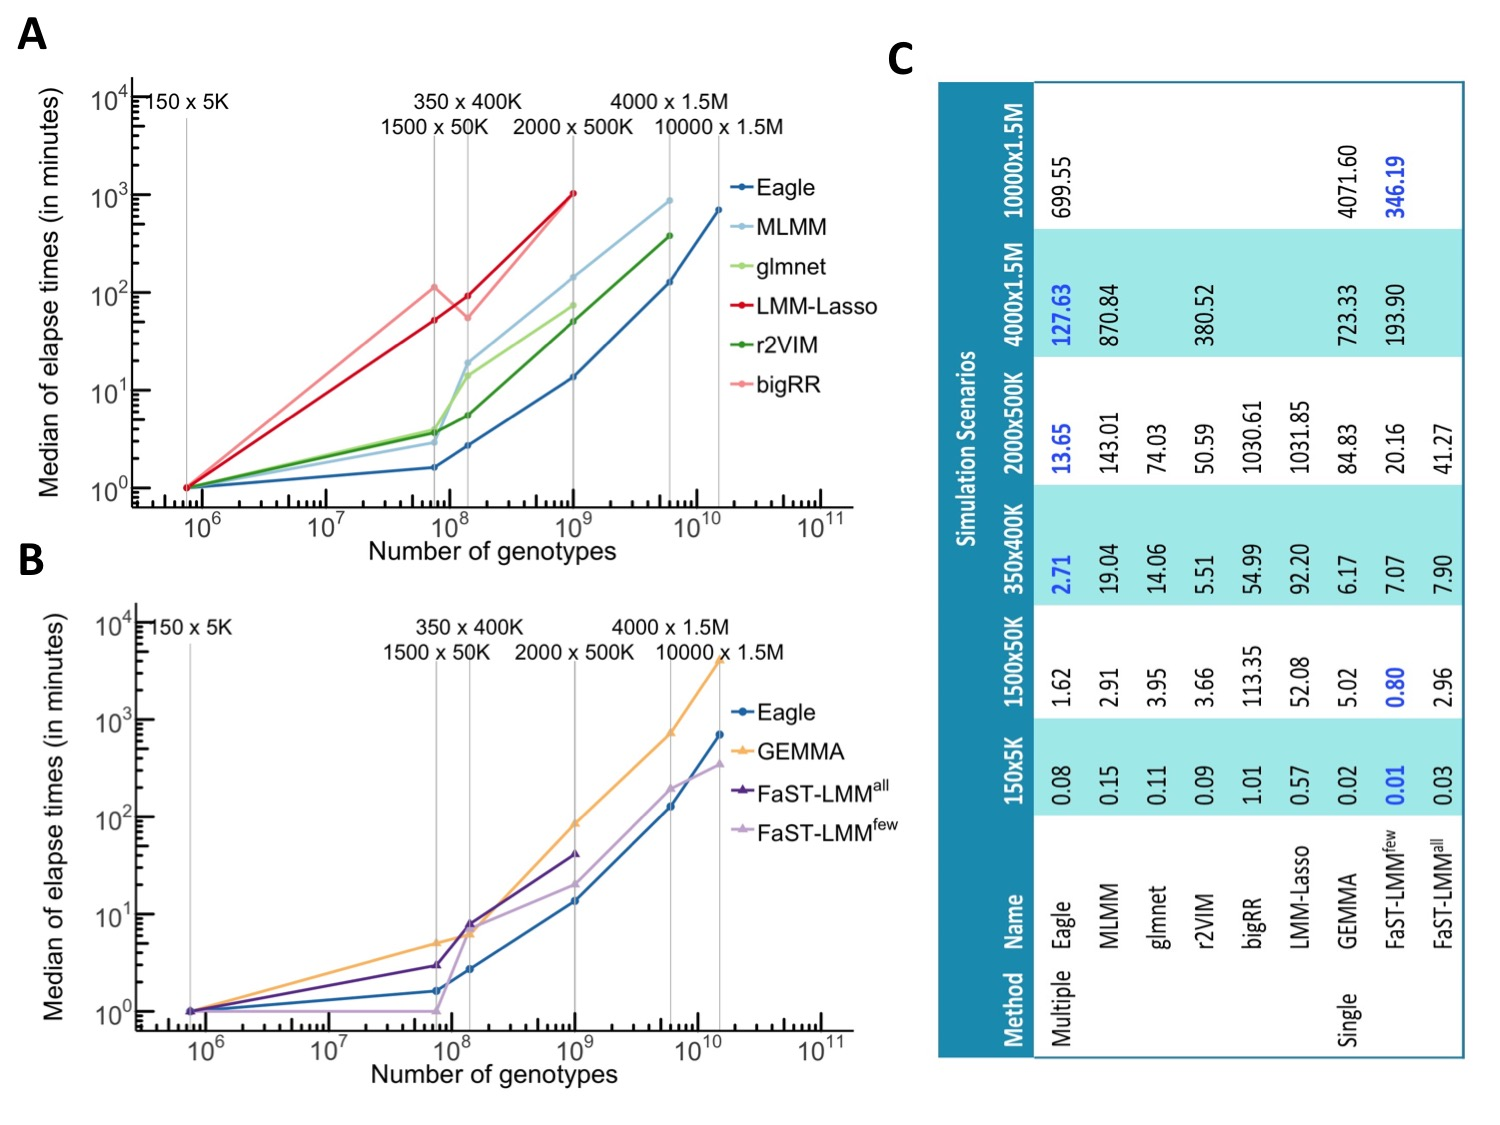
\includegraphics[width=1.2\textwidth,natwidth=610,natheight=642]{Figure2_time.jpg}
\end{figure}

 






\subsection{Mouse Data Analysis}


We were interested in comparing results from Eagle with those from single-locus association mapping for a real data set.
 We chose to focus on data from a large outbred mouse study \citep{nicod2016genome}. This study was unusual in that it collected and analysed SNP dosages (continuous values from zero to one of expected allele counts)  instead of the more common SNP genotypes. Analyses based on dosages rather than discrete genotypes have been shown to have greater power for the detection of genes that are influencing a trait  \citep{zheng2011comparison}. By converting the dosages into genotypes and analysing the data with the single-locus program FaST-LMM, we obtained a subset of those findings reported in the original study. We then analysed the data with Eagle. Due to Eagle's increased power, we found SNP-trait associations not found with  FaST-LMM. However, we were 
 able to confirm the validity of these new findings as they matched what was found in the original study. Having the ability to confirm new findings  in a real study was 
 one of the primary motivators for choosing these data for analysis. 

We repeated the single-locus analyses as first performed \citep{nicod2016genome}, except 
that we focused on autosomal SNPs and our analyses were based on SNP genotypes  rather than SNP dosages. 
In the original analysis, a genome-wide threshold that gave a false discovery rate of 5\%, was found via permutation. We followed the 
same empirical procedure but increased the number of permutations from 100 to 500 for more accurate thresholds.  


We ran Eagle in three ways. 
Eagle chooses the best model via the extended Bayesian information criteria (extBIC) \citep{chen2008extended}. 
  The conservativeness of the extBIC can be adjusted by a single regularisation parameter  $\gamma$ that ranges from zero to one. 
In the simulation study, this parameter was set to one, its most conservative and default setting. The mouse data were also analysed 
under this setting (Eagle$^{default}$).  An alternate  \citep{chen2008extended} , less conservative way of setting $\gamma$ is to  let $\gamma = 1 - \frac{1}{(2\kappa)}$ with $\kappa=\frac{log(L)}{log(n_g)}$ where 
 $L$ is the number of loci that span the genome, and $n_g$ is the number of individuals/groups/lines/strains in the study
  (Eagle$^{alt}$). However, our preferred way is to set the $\gamma$ parameter for each trait via permutation (Eagle$^{optimal}$).  We used 100 permutations to set $\gamma$ to give a false  positive rate of 5\%.  This only took six times as long as a single analysis of the data. This is because the marker data need only be read  once, 
 and only the trait data changes across permutations leading to other computational efficiencies.  
  This permutation method has been implemented within the
 Eagle package. 
  
  
The genome wide results from the analyses of the mouse data are shown in Figure  \ref{figmouse}. The mouse study recorded
measurements on 200 traits. Of these, in the original study, 45 were able to have their findings  corroborated by previously published work. We focused 
our analyses here on these same 45 traits. Overall,  FaST-LMM, Eagle$^{default}$, Eagle$^{alt}$, and Eagle$^{optimal}$ found 50, 37, 67, and 106, SNP-trait findings, respectively, across 39 traits. No associations were found by FaST-LMM and Eagle for the other six traits. 
Eagle$^{alt}$ and Eagle$^{optimal}$ also found SNP-trait associations not found in the original study. This is despite their analyses being based 
on the SNP genotype data and the original study being based on SNP dosage data. Eagle$^{alt}$ found two  and 
Eagle$^{optimal}$ found seven new findings (Supplementary Table \ref{suptabnew}).  These new findings all involved SNPs whose association had been confirmed for other related traits in the original 
study. 

In the simulation study, Eagle outperforms single-locus association mapping. Here, Eagle$^{default}$, where $\gamma=1$, finds less associations 
than FaST-LMM. Why the discrepancy in performance?   The answer lies in the conservativeness of Eagle.  With the added genetic complexity implicit within the mouse data, Eagle is more conservative when $\gamma$ is set to one than in the simulation study.  However, the relative results of the simulation study remain true. For similar false discover rates, Eagle is superior to single-locus association mapping. As a case in point, here FaST-LMM found 50 SNP-trait associations with a false discovery rate of 5\%. Eagle, with the same false discovery rate (Eagle$^{optimal}$) found 106 SNP-trait associations, more 
than a 100\% increase in findings. 







\begin{figure}
\caption{
\setstretch{1.6}{
Genome-wide association mapping results from analyses of the mouse data for the single-locus method FaST-LMM and the 
multi-locus method
Eagle. Eagle was run under three settings; its default setting (Eagle$^{default}$),  an alternate less conservative setting based on 
the number of SNPs and sample size (Eagle$^{alt}$), and where the model selection had been optimised for a false positive rate 
of 5\% (Eagle$^{optimal}$).  The number of SNP-trait associations found are reported in the cells. }
}
\label{figmouse}
\begin{center}
%% obtained from bracewell by running ResultsV2.R from /data/geo047/MWAM/Mouse/OutBred/RScripts/
\includegraphics[width=15cm, height=15cm]{mouseresults.eps}
\end{center}

\end{figure}




 
\section{Discussion/Conclusion}
Eagle is a new linear mixed model based method (and R package) for multi-locus association mapping. It advances the state of association mapping in several ways. 
First, its computational footprint is much smaller than other multi-locus implementations. Eagle makes multi-locus analysis 
practical, even when the datasets are large. Second, the results from
 Eagle are immediately interpretable. They are the set of SNPs in strongest association with the trait where 
each SNP identifies a separate genomic region of interest. Third, it treats association mapping as a model selection problem, avoiding 
 multiple testing issues. 
 As we saw in the simulation study, Eagle has considerably higher power than single-locus methods but is comparable in run time.
Also, when analysing the mouse data, Eagle found more than double the SNP-trait associations than 
with single-locus association mapping, the method of choice. Furthermore, these extra findings were all true. 

Eagle outperformed the other multi-locus methods in our simulation study. However, we are cognisant of the fact  that we made several implementation 
choices that impact our conclusions.  For instance, we chose to calculate the significance of the 
SNP effects from bigRR, LMM-Lasso, and glmnet via stability selection.  Permutation and its variants \citep{ browning2008presto,pahl2010permory} are also equally valid empirical approaches. Stability selection though has the advantage of being based on repeated sampling of only a proportion (50\% in our case) of the 
data. Also, when analysing the (sub)samples, it was not necessary to calculate the entire solution path for a method. 
 Instead,  analyses are 
performed for a fixed value of the regularisation parameter, greatly reducing the amount of computation required. For r2VIM, an R package 
implementing random forests, we had to decide on the  minimum size of a terminal node, the number of trees, and number of potential variables. 
The setting of these parameters greatly affects performance.  We  acknowledge that in the hands of an expert, 
r2VIM could be fine-tuned for a better balance of computational and statistical performance. 
However, we would like to think that the parameter settings we used are sensible 
since they match the values in the original r2VIM publication \citep{szymczak2016r2vim}.



Eagle's computational speed does come at a cost. It is a weakness shared by all of the methods considered here, although in different ways. 
Eagle cannot handle extra random effects which are sometimes needed when more advanced study designs are employed. One solution 
is to adopt a two-stage analysis procedure. In the first stage, a single linear mixed model is fitted to the data. Much of the modelling complexity, 
including the extra random effects, is 
captured in this first-stage model. In the second stage, Eagle is run not on the original trait data but adjusted trait data which are obtained from the first stage analysis. Even though this is a well accepted practice, it is approximate \citep{gogel2018comparison}.  A better solution is to fit a single model to the data. 
Although not specifically designed for association mapping,
WGAIM \citep{verbyla2007analysis}, upon which Eagle is based, and RWGAIM \citep{verbyla2012rwgaim}  are two R packages where this is possible. The difficulty is that for large datasets and/or complex 
models,  run time and memory usage can become limiting factors for analysis. 


Over the coming years, computationally, the demand placed upon association mapping methods is going to increase. 
High-throughput array-based technologies continue to decrease the cost of genotyping, permitting ever larger GWASs to be performed. 
Whole-genome sequencing is also now a reality. Already sequence across entire genomes are being collected for GWASs \citep{gudbjartsson2015large, long2017whole}
culminating in data on millions of SNPs. It is because of this growing demand that 
we have purposely structured the Eagle package for continued development. We are already experimenting with a GPU-based version of Eagle. 
Early results suggest that for small to moderate sized datasets ($<$10,000 samples), there is little improvement in performance over CPU-based 
computation.  However, for larger study sizes, we are seeing up to a 40\% decrease in run times.  
We also have plans for Eagle to run on computer clusters. Structuring Eagle for larger-than-memory calculations was a 
preemptive step in this direction. GWASs have changed significantly in the past decade but the size and complexity of GWASs is expected 
to change even more in the coming decade. 





\section*{Data Availability}
The input files for Eagle containing the mouse GWAS data are available for download from 
https://doi.org/10.25919/5bc08287717dd. The original data were obtained from the Heterogeneous Stock Mice website 
http://wp.cs.ucl.ac.uk/outbredmice/heterogeneous-stock-mice/.  



\section*{Acknowledgements}
We would like to thank the IM\&T Scientific Computing group at the Commonwealth Scientific and Industrial Research Organisation (CSIRO) for providing access and support to the CSIRO Accelerator Cluster upon which all computation was performed. 



\section*{Funding}
This research received no specific grant from any funding agency in the public, commercial, or not-for-profit sectors.

\vspace{1cm}
\noindent
{\em Conflict of interest:} The authors declare that they have no
competing financial interests.





  
 


%%\bibliographystyle{naturemag}
\bibliography{biblibrary}


\end{document}
